\documentclass[11pt]{article}
\renewcommand{\baselinestretch}{1}
\usepackage[utf8]{inputenc}
\usepackage[parfill]{parskip}
\usepackage{graphicx}
\usepackage{amsmath}
\usepackage{caption}
\captionsetup[table]{position=bottom} 
\usepackage[title]{appendix}
\usepackage[margin=25mm]{geometry}
\usepackage{amsmath,graphicx,psfrag,pstricks}
\def\n{\noindent}
\def\u{\underline}
\usepackage{gensymb}
\def\hs{\hspace}
\newcommand{\thrfor}{.^{\displaystyle .} .}
\newcommand{\bvec}[1]{{\bf #1}}
\usepackage{graphicx}
\usepackage{rotating}
\graphicspath{{Plots/}}
\usepackage{amsmath}
\usepackage{booktabs}
\usepackage{siunitx}
\usepackage{amssymb}
\usepackage[utf8]{inputenc}
\usepackage[justification=centering]{caption}
\usepackage{float}
\usepackage{listings}
\usepackage{color} %red, green, blue, yellow, cyan, magenta, black, white
\definecolor{mygreen}{RGB}{28,172,0} % color values Red, Green, Blue
\definecolor{mylilas}{RGB}{170,55,241}
\lstset{language=Matlab,%
    %basicstyle=\color{red},
    breaklines=true,%
    morekeywords={matlab2tikz},
    keywordstyle=\color{blue},%
    morekeywords=[2]{1}, keywordstyle=[2]{\color{black}},
    identifierstyle=\color{black},%
    stringstyle=\color{mylilas},
    commentstyle=\color{mygreen},%
    showstringspaces=false,%without this there will be a symbol in the places where there is a space
    numbers=left,%
    numberstyle={\tiny \color{black}},% size of the numbers
    numbersep=9pt, % this defines how far the numbers are from the text
    emph=[1]{for,end,break},emphstyle=[1]\color{red}, %some words to emphasise
    %emph=[2]{word1,word2}, emphstyle=[2]{style},  
}
\title{Part IIA Project - GF1: Control Systems - First Interim Report}
\author{Bailey Brookes | Corpus Christi | bdb31}
\date{\today}

\begin{document}
\maketitle

\section{Subsystems}
\subsection{Evaporator}
Due to the evaporator having derivatives in its equation, design is done by first taking Laplace transforms of the equations, revealing that there are two integrators. Therefore overall the system has 3 states, one in the separator and two in the condenser.

To test the evaporator subsystem, step inputs are placed at all inputs and outputs measured after a certain simulation time. This simulation time is found by considering the two negative feedback loops which both contain integrators. The negative feedback makes the system stable, and constant F1 and F2 make the system stable as product blocks act as gains. Using this gains the time constants for each loop can be found by considering each loop as a integrator with gain $k$ and negative feedback. The transfer function for such a system is $G(s) = \frac{s}{s+k}$ with pole $-k$  and time constant $\frac{1}{k}$. So for the X2 and P2 loops:

\begin{itemize}
\item X2 Loop has loop gain (pole) $0.05$ and a time constant of 20 
\item P2 has loop gain (pole) $2.5527 \times 10^{-4}$ and time constant $3917.42$ 
\end{itemize} 

So the simulation should be run for a duration a couple times bigger than the largest time constant. The plots of some of the outputs are show in Figures \ref{P2}, \ref{X2} and \ref{F4}, showing the model is stable.

\subsubsection{Linearising the Evaporator}
Simulink allows non linear models, such as the evaporator, to be linearised using linmod. This gives the state space model of the linearises system, which is:

\[
A = 
\begin{bmatrix}
-0.05 & 0 \\
-0.0001 & -0.0003
\end{bmatrix}
\hspace{1cm}
B = 
\begin{bmatrix}
0.0500 & 0.0500 & -1.2500 & 0 & 0 & 0\\
-0.0380 & 0 & 0 & -0.2500 & 0.0005 & 0.0065
\end{bmatrix}
\]
\[
C = 
\begin{bmatrix}
    1.0000&         0\\
         0&    1.0000\\
         0&    0.5070\\
    0.3126&    0.5616\\
   -0.0006&   -0.0010\\

\end{bmatrix}
\hspace{2cm}
D = 
\begin{bmatrix}
0&         0&         0&         0&         0&         0\\
0&         0&         0&         0&         0&         0\\
0&         0&         0&         0&         0&         0\\
0&         0&         0&         0&         0&         0\\
-0.1520 &        0&         0&         0&    0.0018&    0.0260

\end{bmatrix}
\]

The eigenvalues of A gives the poles of the linearised system, which are -0.0003 and -0.05. This gives us an additional two checks to the model: 
\begin{enumerate}
\item These poles should correspond to the time constants calculated before. Time constants for these two poles are 3333.33 and 20, with the difference between the larger value down to rounding errors in matlab.
\item Changing F1 by a factor of 10 should make the P2 loop 10 times faster, so the pole (eigenvalue should be one tenth the size. Both the simulink and analytical shows that this is the case, with the system having time constant 33333.33 in simulink and 39174.2077 analytically.
\end{enumerate}

\subsection{Condenser and Steam Jacket}
Both the condenser and the steam jacket where designed directly from there equations given in the handout and these systems are shown in Figures \ref{condenser} and \ref{steamjacket} respectively. Complete models of the separator and evaporator depicted in the handout are omitted from the appendix for conciseness.

\section{Whole Process}
\subsection{Test Results}
Testing and debugging revealed one floor in the initial design, that divisor blocks had been used wrong in the condenser, affecting output to all other subsystems. Once the ports had been switch round for these blocks throughout the system, the process's nominal values where reached. 

\subsection{Trim Results}
Another method of testing the systems steady state is the trim function in simulink. A trim/equilibrium point is a point in the parameter space of a dynamic system at which the system is in a steady state. That is, when the system's state derivatives equal zero. For this model, these points should be the same as the nominal values given in the handout, with some rounding error. These results from the trim function in simulink are tabulated below.
\begin{table}[H]
\centering
\label{my-label}
\begin{tabular}{|cc|}
\hline
Output & Value    \\ \hline
X2     & 25       \\
P2     & 50.5053  \\
T2     & 84.6088  \\
F4     & 8        \\
F5     & 8        \\
Q200   & 308.0002 \\
T201   & 46.1539  \\
T100   & 119.9449 \\
Q100   & 339.2263 \\
F100   & 9.2685   \\
L2     & 0        \\ \hline
\end{tabular}
\caption{Trim analysis results}
\end{table}

\appendix
\section{Plots of the evaporator response}

\begin{figure}[H]
\centering	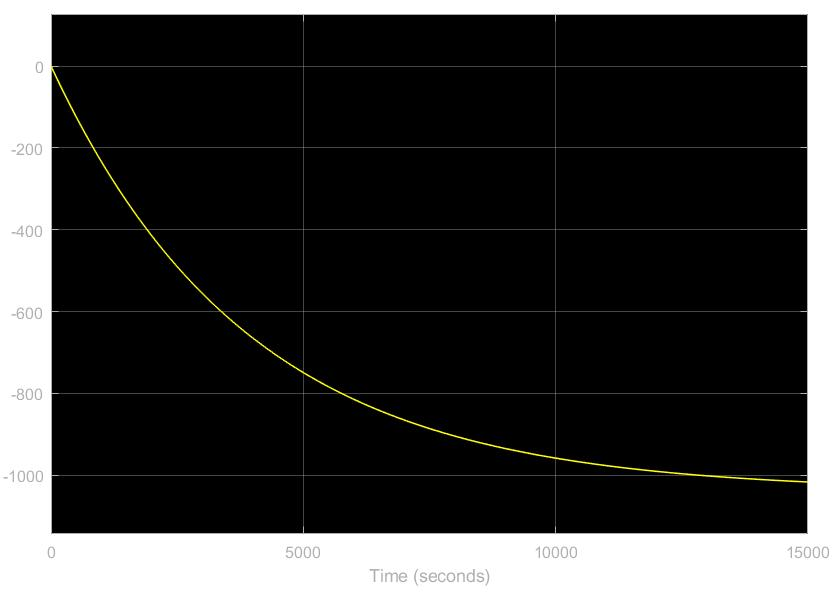
\includegraphics[scale = 0.4]
{P2_15000}
\caption{Response of P2}
\label{P2}
\end{figure}

\begin{figure}[H]
\centering	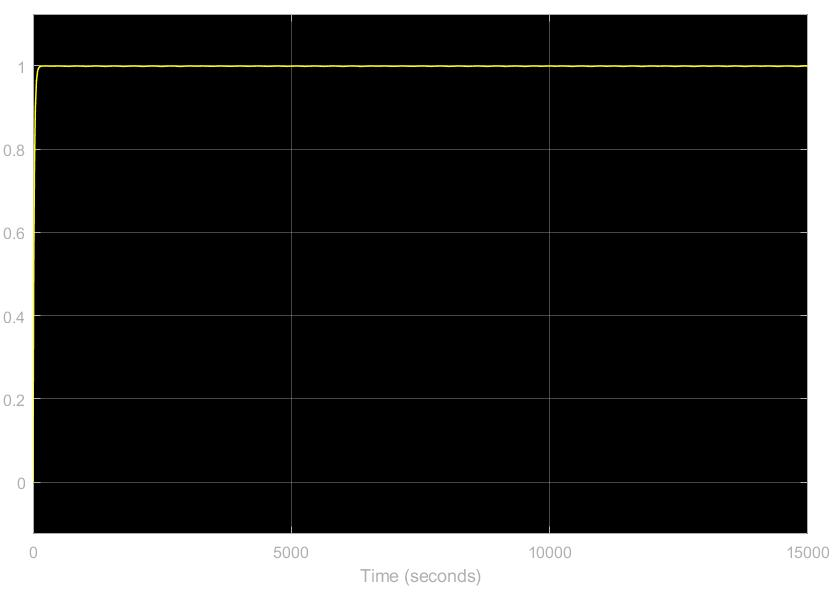
\includegraphics[scale = 0.4]
{X2_15000}
\caption{Response of X2, which is much faster than that of P2, as in seen by the very sharp rise at the start}
\label{X2}
\end{figure}

\begin{figure}[H]
\centering	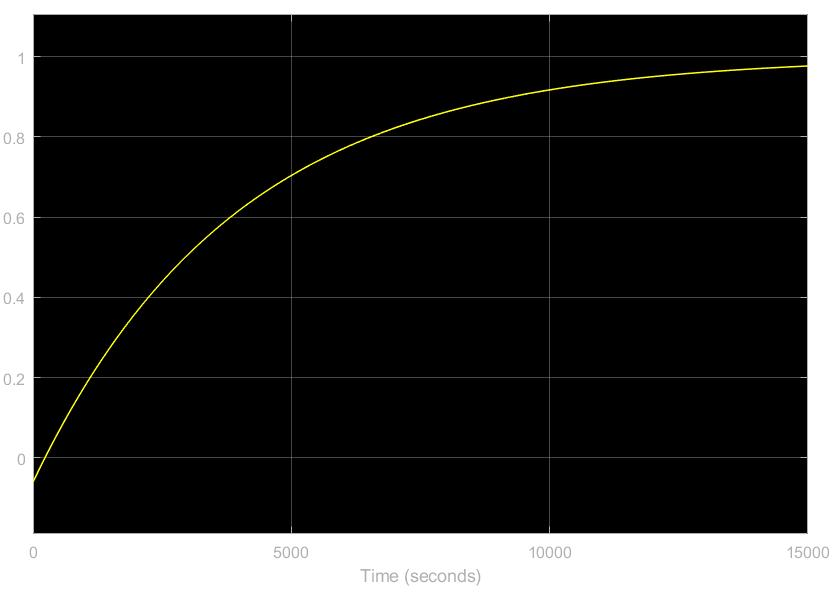
\includegraphics[scale = 0.4]
{F4_15000}
\caption{Response of F4}
\label{F4}
\end{figure}

\section{Subsystems}

\begin{figure}[H]
\centering	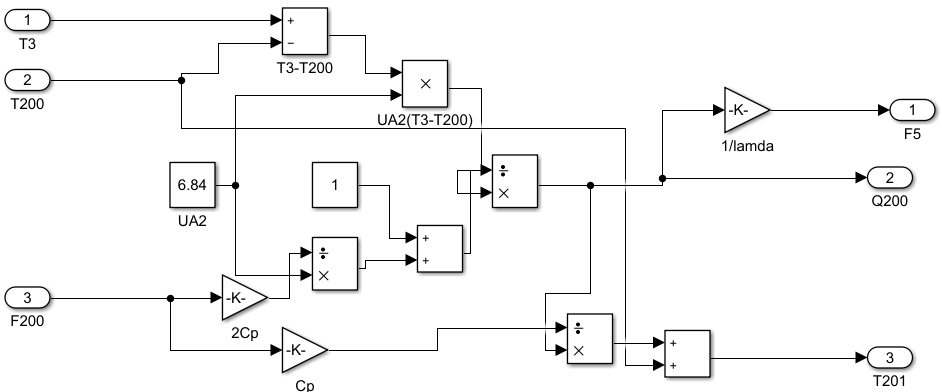
\includegraphics[scale = 0.8]
{condenser}
\caption{Condenser Model}
\label{condenser}
\end{figure}

\begin{figure}[H]
\centering	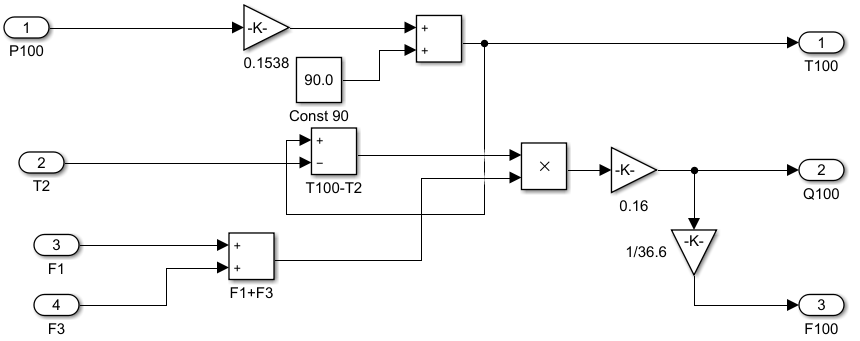
\includegraphics[scale = 0.8]
{steamjacket}
\caption{Steam Jacket Model}
\label{steamjacket}
\end{figure}

\section{Complete Model}
\begin{figure}[H]
\centering	\includegraphics[scale = 0.6]
{Process}
\caption{Model of entire process}
\label{process}
\end{figure}

\end{document}